\chapter{急性关节痛}

急性关节痛是急性关节炎的主要症状。急性关节痛可由关节内(包括软骨、骨质、滑膜)的病变和关节周围的肌腱骨附着点炎症(血清阴性脊柱关节病的基本病理变化)所致。另外,关节周围组织急性炎症(如滑囊炎、腱鞘炎、肌纤维组织炎)也可被患者主诉为急性关节痛。

急性关节炎起病急骤,常表现出关节急性炎症的特点,如红、肿、热、痛与功能障碍。在急性炎症时局部皮肤还常有肿胀、潮红、发热和运动受限等病征。由于引起关节炎症的原因很多,而临床表现很相似,常常造成诊断和鉴别诊断上的困难。但通过详细的病史、局部和全身体格检查,以及有关的实验室检查和影像学检查,多可获得正确的诊断。

病史对于关节病的病因分析很重要,需详细询问患者关节病变发生、发展的过程、起病急或缓、疼痛的部位、疼痛的程度、与天气的关系、日夜间的差别、有无原发病灶以及全身性疾病等。当患者罹患败血症或某些急性传染病时,或在关节腔内注射药物后而出现关节红、肿、痛,应考虑感染性关节病变;急性关节炎起病前1个月内有急性腹泻史,应注意肠病型的Reiter(莱特尔)综合征;急性关节炎伴有尿道感染或子宫颈炎,则应注意性病型的Reiter综合征;夜间关节痛加重,晨起时关节疼痛、僵硬更加明显者,尤应注意类风湿关节炎和血清阴性脊柱关节病;久坐或固定某一体位(如长时间驾驶、长时间使用电脑)后症状加重,活动后症状减轻者,应注意强直性脊柱炎;行走和上、下楼关节痛加重,休息后好转,提示骨性关节病,而休息不好转、活动后症状改善者,则多是自身免疫介导的关节病变。

体格检查必须系统地进行,例如先从颈椎、胸椎及腰椎顺序开始,然后颌部、肩部、上肢、骨盆及下肢。应注意病变是单关节或多关节,两侧关节外形是否对称,肢体的位置,周围肌肉有无紧张或萎缩,局部皮肤有无红、热,关节有无肿胀、压痛、波动感,站立、行走的姿势,以及运动范围的测定等。单关节病变须警惕感染性关节炎,足部急性单关节炎则要注意痛风性关节炎的初次发作。急性单关节炎还常见于反应性关节炎(属于“血清阴性脊柱关节病”的范畴)。

4字试验:患者仰卧,健侧下肢伸直,患侧髋、膝关节屈曲外展外旋,足置于健侧大腿上,检查者一手压在健侧髂前上棘以固定骨盆,另一手在屈曲的膝部下压,若此时臀部发生疼痛,即为试验阳性。本试验阳性多提示骶髂关节的炎症,结核或股骨头坏死等病变。

浮髌检查:患者平卧,患肢伸直放松。检查者左手将髌骨上方的髌上囊内液体向下挤压入关节腔,右手食指将髌骨下压,一压一放,反复数次。如关节腔内有大量积液,食指迅速放开时髌骨立即浮起,食指可感到明显的浮动感,称浮髌现象。出现浮髌现象提示关节腔内有积液。

实验室检查对鉴别诊断甚为重要。血沉和C反应蛋白是非特异性的炎症指标,这两项指标的测定有助于区别关节病变是炎症或非炎症性。自身免疫介导的风湿性疾病的关节炎,多有较明显的血沉和C反应蛋白增高;慢性感染性关节炎,如结核性关节炎也伴血沉和C反应蛋白明显增高;急性化脓性关节炎往往C反应蛋白增高比血沉增高更明显。骨性关节炎(退行性关节病变)继发滑膜炎时血沉和C反应蛋白轻度增高,痛风性关节炎也多是血沉和C反应蛋白轻度增高。大部分骨性关节炎血沉和C反应蛋白不高,肥大性骨关节病、关节血肿、神经源性关节病则血沉和C反应蛋白往往正常。此外,血沉和C反应蛋白还可反映关节炎症为活动性或非活动性,血沉和C反应蛋白持续增高说明关节炎症仍有活动,血沉和C反应蛋白趋向正常反映关节炎症趋于非活动性,但血沉和C反应蛋白与强直性脊柱炎的活动性无明显相关性。此外,不少并存疾病可引起血沉或C反应蛋白增高,所以有必要除外这些情况,方有诊断参考价值。

血清类风湿因子(RF)以及抗环瓜氨酸肽(CCP)抗体测定对类风湿关节炎的诊断有重要的意义,尤其是抗CCP抗体。类风湿因子明显增高对类风湿关节炎有较高的敏感性和一定的特异性,其阴性不能成为排除类风湿关节炎的依据,因为约有30\%的类风湿关节炎始终表现为类风湿因子阴性。类风湿因子轻度增高者,还需注意红斑狼疮、干燥综合征等其他结缔组织病。而CCP抗体与RF相比,具有更好的特异性,且可在关节炎早期出现。此外,其对疾病预后的判断具有重要的价值。

抗核抗体谱(ANAs)检查对结缔组织病的关节炎有鉴别诊断价值。在临床上ANA检测实际上是指总抗核抗体的检测,是结缔组织病的一项极其重要的筛选试验。较高浓度的抗核抗体(ANA)阳性提示结缔组织病的存在,但不能确定是哪一种结缔组织病。抗ds-DNA抗体对红斑狼疮的诊断有高的特异性;抗SSA(Lo)抗体和抗SSB(La)抗体阳性提示干燥综合征;抗Jo-1抗体阳性提示皮肌炎和多发性肌炎;抗Scl-70抗体阳性提示硬皮病(系统性硬化症);抗ul-RNP抗体阳性提示混合性结缔组织病;抗PM抗体阳性多提示多发性肌炎和系统性硬化症重叠。由于红斑狼疮可以出现上述任何一个抗体阳性,所以如果抗核抗体和抗ds-DNA抗体均阳性的同时有其他抗体阳性,诊断上还是考虑红斑狼疮为主。但如果红斑狼疮患者抗SSA抗体或抗SSB抗体阳性,则患者常伴有口干或眼干症状;如果红斑狼疮患者抗ul-RNP抗体阳性,则常常伴有较明显的雷诺现象。

强直性脊柱炎和其他脊柱关节病患者常常伴有较高的HLA-B27阳性率,因此有脊柱关节病症状者如果HLA-B27阳性,则增加一个诊断的支持点,但其诊断仍是以骶髂关节的放射学改变为诊断的必备条件。

血清抗链球菌溶血素“O”(ASO)滴度测定增高提示有链球菌感染史,需要警惕风湿热。此外,抗DNA酶B、抗透明质酸酶抗体、抗链球菌激酶抗体、抗核苷酸酶抗体的测定也具有其必要性。如果患者符合风湿热的诊断标准,应该诊断为风湿热;如果急性关节炎之前有明确的链球菌感染病史,则考虑为链球菌感染后反应性关节炎。临床上不应草率地下一个所谓的“风湿性关节炎”,以免延误原发病的诊断和治疗。

血尿酸增高以及关节炎发作时滑液培养阴性对痛风性关节炎的诊断有重要意义。

X线检查可以观察关节面、关节腔、关节周围软组织和骨质等变化,但许多急性关节疾病的X线平片检查常无明显改变,故X线检查对慢性关节病的诊断意义较大。CT、MRI检查对于关节的早期病变往往具有很好的判断价值。

关节腔穿刺液检查时,积液的颜色、蛋白含量、红细胞数、白细胞数和分类、涂片有无细菌、细菌培养以及动物接种等,对各种类型关节炎的鉴别诊断有一定意义。

关节镜可直接观察滑膜、软骨、半月板与韧带的形态结构,并可对病变组织取活检。针刺活检是一种操作简单、创伤小的检查方法,通过穿刺取滑液和滑膜,便于快速诊断。关节穿刺术或关节滑膜活检要严格遵守无菌操作常规,以免引起关节附加感染。

根据临床病变经过的不同,关节疾病可分为急性与慢性两大类,但急性关节炎可发展为慢性关节炎,而不少慢性关节炎亦有急性发作的表现,在鉴别诊断时应互相参考。能引起急性关节痛的有下列各种疾病见表\ref{tab42-1},分别讨论如下。

\begin{table}[htbp]
\centering
\caption{急性关节痛疾病的分类}
\label{tab42-1}
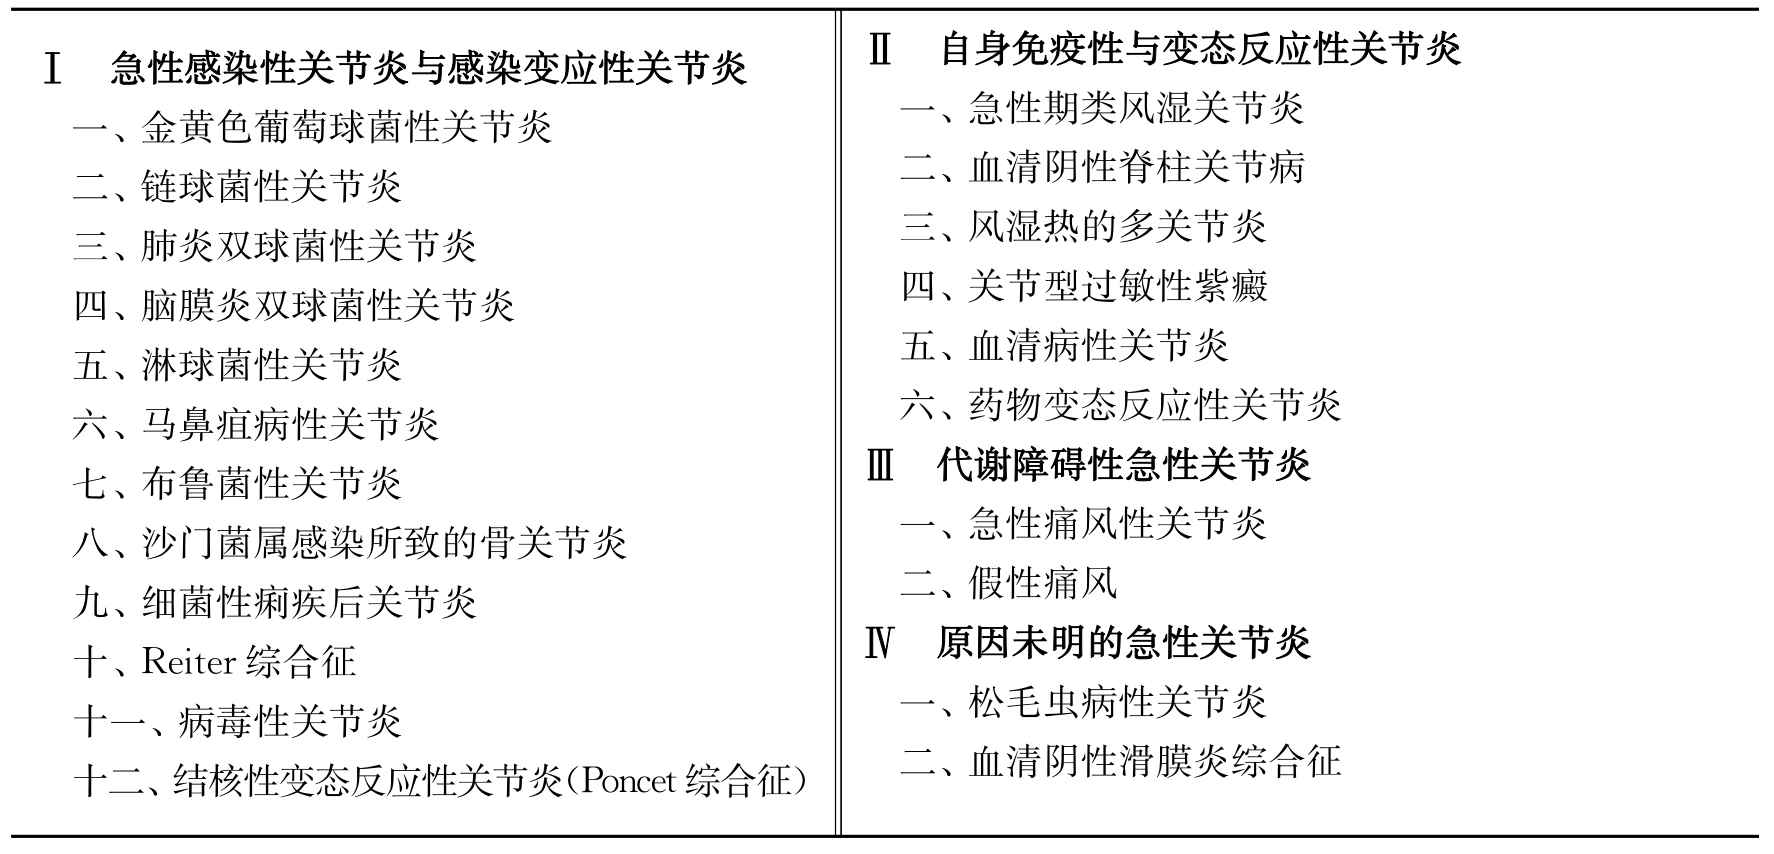
\includegraphics[width=5.90625in,height=2.83333in]{./images/Image00254.jpg}
\end{table}

\protect\hypertarget{text00323.html}{}{}

\section{139 急性感染性关节炎与感染变应性关节病变}

此类关节病变具有两种情况:一种是细菌直接侵袭关节引起关节化脓,患者的关节穿刺液涂片及细菌培养均阳性;另一种是由于细菌的毒素或代谢产物所致的变态反应性关节病变,其关节腔穿刺涂片和细菌培养均阴性,如猩红热、波状热、痢疾后引起的反应性关节炎等。

由于抗生素的广泛应用,临床上急性化脓性关节炎已经少见,感染变应性关节炎的种类也有变化,过去链球菌感染后反应性关节炎常见,而今痢疾后和尿路感染后反应性关节炎更常见。

\subsection{一、金黄色葡萄球菌性关节炎}

急性化脓性关节炎的病原菌最多为葡萄球菌,尤其是金黄色葡萄球菌,可发生于任何年龄,但以儿童为多见。可继发于金黄色葡萄球菌败血症,但也可由邻近的骨髓炎或软组织感染蔓延,或关节外伤细菌直接侵入所致。病变常侵犯单个大关节,以髋关节最多见,其次是膝关节、肩关节,偶见多关节的化脓性关节炎。

化脓性关节炎首先是滑膜炎,滑膜迅速肿胀、充血、白细胞浸润与关节腔渗液,关节囊及其周围组织有蜂窝织炎或脓肿形成。临床上有如下特点:①起病急骤,常有明显的恶寒或寒战,体温迅速上升,可达39~40℃,血象中性粒细胞明显增多;②任何关节均可受累,以负重关节如髋和膝关节受累最多,多侵犯单关节,特征是受累关节灼热、疼痛剧烈、肿胀明显、活动障碍,较表浅的关节可有波动感,多半因肌肉痉挛使关节处于半屈位置(化脓性髋关节炎时,患肢常处于外展、外旋、前屈位);③关节腔穿刺液为脓性渗出液,涂片白细胞增多,由数千~10万个/
mm\textsuperscript{3}
,90\%以上为中性粒细胞,涂片染色检查或培养可发现大量金黄色葡萄球菌。

关节腔穿刺液涂片染色检查或培养发现金黄色葡萄球菌是本病的最重要诊断依据。但有时可与邻近关节的急性骨髓炎相混淆。骨髓炎的压痛点局限于干骺端而不在关节,关节虽也可有肿胀,但关节本身体征较微,渗出液培养阴性,与本病不同。本病还需与急性痛风性关节炎区别;患者缺乏痛风性关节炎的症状,血尿酸正常,均易于除外急性痛风性关节炎。另外,由于关节腔内注射肾上腺皮质激素治疗过程中的污染,引起关节化脓者也不少见。

\subsection{二、链球菌性关节炎}

链球菌性关节炎最多并发于猩红热。猩红热多发生于儿童,其临床特点为突然高热、咽峡炎、弥漫性猩红色皮疹,继而脱皮。可出现关节、心脏、肾脏的并发症。猩红热性关节炎一般可区分为下列两型:猩红热败血症性关节炎与猩红热变态反应性关节炎。

猩红热败血症性关节炎是由于乙型溶血性链球菌侵入关节所引起,罹患关节的表现与化脓性关节炎相同。由于青霉素治疗的普遍应用,此型关节炎已罕见。猩红热变态反应性关节炎是少见的并发症,有人称之为“猩红热性风湿病”,多发生于普通型猩红热。山西等地2235例猩红热中,并发此型关节炎者有40例,占1.8\%。关节症状多在病程第一周后出现,大小关节都可累及,以下肢关节较多。病变为多发性、游走性,关节有红、肿、痛,但不化脓,症状经数天消失。这类关节炎现在多被称为链球菌感染后反应性关节炎。

在亚急性感染性心内膜炎时(多数由草绿色链球菌与溶血性链球菌引起),短暂的关节痛较为常见,特别是在起病时,但极少引起化脓性关节炎。对于链球菌感染后引起的非化脓性关节炎,称为链球菌感染后反应性关节炎。

\subsection{三、肺炎双球菌性关节炎}

本病是一种急性化脓性关节炎,主要发生于婴儿。如关节炎继发于肺炎,关节症状常在肺炎发病两周之后出现。本病好侵犯髋关节,脓液稠厚,不易抽出,易遗留关节强直。这类关节炎在医疗条件比较好的城市和地区已经非常罕见。

\subsection{四、脑膜炎双球菌性关节炎}

关节炎为流行性脑膜炎(流脑)较常见的并发症,可见于5\%的病例。国内报告的一组病例中,以单发性关节炎为多见,多侵及大关节。以肘、膝、踝、腕关节最为多见。关节炎大部分发生在体温降至正常之后,当关节炎出现时,体温又再上升。通常表现为感染变应性关节炎,罹患关节疼痛、水肿及运动受限制,但很少发红,经过短暂,预后良好。脑膜炎双球菌性关节炎的关节化脓罕见,此病以形成脓性渗出液为特征,渗出液中含大量脓细胞,并可找到脑膜炎双球菌。

\subsection{五、淋球菌性关节炎}

淋球菌性关节炎是由淋菌或其毒素侵入关节腔所引起,由淋菌直接引起者是化脓性关节炎,常为单发性,最后可致关节强直。由淋菌毒素所引起者为变态反应性炎症,通常侵犯多个关节,在淋病任何时期均可发生。

淋菌性化脓性关节炎病变常波及膝、踝、肘、肩等大关节,较特别者有时可侵犯下颌关节,以致进食困难。此病的主要诊断根据是:①患者有泌尿生殖系淋病;②起病急骤,受累关节肿胀、疼痛、潮红、灼热与功能障碍;③非甾体抗炎药不能控制病情,但磺胺类及青霉素类抗生素治疗有效;④在关节腔内脓性渗出液中可找到淋菌。

\subsection{六、马鼻疽病性关节炎}

人类的马鼻疽病少见,患者都有与病马直接或间接接触史。临床上以发热、脓疱疹、深部肌肉有肉芽肿性疖肿和关节痛为特征。1961年报告18例中,12例有关节炎症改变,轻者仅有关节酸痛,重者有关节肿胀,痛较剧烈,甚至运动障碍,最常受累的是踝、膝与肩关节。

\subsection{七、布鲁菌性关节炎}

布鲁菌病是一种急性、亚急性或慢性全身性感染疾病,临床上以波状热型、多汗、疲乏和关节痛为特点。多并发变态反应性关节炎,仅有少数发生化脓性关节炎。常见的关节病变是滑膜炎、关节周围炎和关节旁软组织炎以及骨关节炎。国内报告一组90例,均有关节疼痛症状。其关节表现的特点为游走性多发性关节炎,主要侵犯大关节,依次为骶髂、髋、膝、肩、腕、肘等关节,指(趾)关节较少受累,与风湿热的多关节炎相似。

\subsection{八、沙门菌属感染所致的关节炎}

沙门菌属中以猪霍乱杆菌感染并发的关节炎最为常见。大多数起病突然,有畏寒、发热、头痛、四肢关节酸痛等中毒症状,伴有轻重不一的胃肠道症状,在病程中或恢复期常出现并发症。国内一组猪霍乱沙门菌感染中,有并发症者高达68.5\%,其中以骨与关节受累者最多见。临床表现以肋骨脓肿及肋骨骨髓炎最多见,或有流脓窦道形成。这种窦道与结核性或化脓性骨关节感染的窦道不同,在应用一些抗生素或休息后可自行愈合。从窦道脓液培养中常可获得猪霍乱沙门菌。关节炎往往为单关节受累,任何关节均可累及,常见于膝、髋关节,表现为关节局部肿胀、疼痛、红热和功能障碍。临床上如血清凝集反应滴度增高或逐周增高,有辅助诊断价值。自骨髓、关节滑膜液、脓液、血液中检出病原菌,可确定诊断。

\subsection{九、细菌性痢疾后关节炎}

痢疾后关节炎偶发生于急性细菌性痢疾发病后2~3周,常侵犯膝、踝、肘、腕等大关节,且为多发性,可以对称性,也可以非对称性。此时患者可再度发热,关节疼痛,关节腔内有浆液性渗出液,经1~2周痊愈。本病是变态反应性关节炎,非细菌直接侵袭引起,关节滑液细菌检查阴性。这类关节炎已多被称为“莱特尔综合征”的肠炎型。

\subsection{十、莱特尔综合征}

典型的莱特尔(Reiter)综合征由包涵体结膜炎衣原体感染所引起,具有非淋病性尿道炎、结膜炎及关节炎三联症,以青壮年男性多见。女性则往往伴有宫颈炎。莱特尔综合征首次发病往往表现为一种急性关节炎,部分患者演变为慢性关节炎,反复急性发作,可迁延数月至数年。莱特尔综合征发病初期常先有尿道炎症状,可并发前列腺炎、膀胱炎,数天后出现结膜炎,少数病例有角膜炎及虹膜炎,继而出现关节症状。关节症状在此三联症中最突出,半数患者可以没有结膜炎。通常在发病后两周内出现急性多发性关节炎,有剧烈疼痛与灼热,甚至肿胀。症状从一个关节开始渐波及其他关节,最常侵犯的是负重的大关节,如膝和踝关节,其他如指、趾、腕、髋、脊椎关节均可累及,最后又固定于一二个关节,如膝与骶髂关节。关节腔渗出液培养阴性,血沉和C反应蛋白增高。部分患者可伴有发热。此病的眼部和尿道症状多在数天至数周消失,但关节炎一般经过2~6个月才痊愈,部分病例可反复复发,致关节症状迁延一至数年之久,往往遗留肌肉萎缩,HLA-B27阳性的患者可发展为强直性脊柱炎。

莱特尔综合征在病程中可在尿道、滑膜液及结膜分泌物中分离出衣原体,血清学检查特异性抗体阳性滴度增高。免疫学研究还证明人类白细胞抗原HLA-B27与莱特尔综合征有关,60\%~96\%的病例为HLA-B27阳性。

\subsection{十一、病毒性关节炎}

某些病毒感染(流行性腮腺炎、腺病毒感染、风疹、病毒性肝炎、登革热、虫媒病毒感染、传染性单核细胞增多症等)可出现多发性关节炎,病变多为自限性,特别多见于病程的前驱期。

风疹可有多发性关节炎的表现,常累及肢体的小关节,罹患者大多为年轻成人,尤以女性居多。关节炎与皮疹同时出现,或稍后于皮疹而出现。关节炎症在两周之内消退,不遗留任何关节损害。

乙型病毒性肝炎也较常并发关节炎。关节炎(有时并发皮疹)可在黄疸发生前数天乃至两周出现,或与黄疸同时出现。关节炎也可见于无黄疸型病例。关节炎为自限性,可累及大、小关节,痊愈后不遗留关节损害。如累及双侧手关节,可误诊为类风湿关节炎。同时可有肝功能异常。在前驱期,血清与关节滑液常可检出乙型肝炎病毒抗原。关节滑膜炎被认为是由于肝炎病毒抗原与抗体的免疫复合物所引起。

\subsection{十二、结核性变态反应性关节炎(Poncet综合征)}

结核性变态反应性关节炎是由结核杆菌毒素引起的机体变态反应,多并发于成人原发性肺结核和淋巴结结核,个别并发于肠结核或肾结核,不属于罕见病例。病因与由结核杆菌直接感染引起的单发性结核性关节炎不同。可以呈急性或慢性,患者大多数为青年,本病急性发作时表现为弛张热或不规则型热、乏力、结节性红斑和关节炎。临床上出现下肢为主的结节性红斑,需警惕结核性变态反应性关节炎。有时以关节症状为主要的临床表现,可以酷似风湿热的多关节炎。往往表现为多发性游走性关节痛,急性期关节有红、肿、热、痛等征象,常由小关节开始,渐而波及大关节,主要为指、腕、膝、踝、肩、腰椎等关节。部分病例仅有关节酸痛。结核性变态反应性关节炎有周期性好转与恶化的特点。

结核性变态反应性关节炎的诊断主要根据以下几点:①患者体内有结核病灶;②出现风湿病样关节症状;③结核菌素试验阳性;④无心脏受累的病征;⑤非甾体抗炎药治疗无效,而抗结核药物治疗有效。

结核性变态反应性关节炎的诊断较难,常误诊为风湿热的多关节炎,据文献报告在一组52例结核性变态反应性关节炎病例中,36例曾被误诊为风湿病而进行抗风湿治疗。因此对已诊断为风湿热的病例,仍需警惕有此病的可能性。凡青年患者,有关节症状及结节性红斑,经充分的抗风湿治疗无效,又无其他疾病可以解释者,应警惕此病,进一步找寻结核病灶,并作结核菌素试验,如为强阳性,说明体内有结核感染,可作抗结核的诊断性治疗。抗结核治疗的反应是诊断本病的重要依据;如治疗后关节症状和发热均消退,诊断可以确定。但抗结核治疗后一般发热消失最快,关节症状与结节性红斑消退较慢;因此,如抗结核治疗后关节症状尚未迅速消退,也不能否定其治疗作用,有怀疑时仍需积极继续抗结核治疗。

本病有慢性复发倾向,其慢性型的经过较缓和,关节痛比其他症状恢复较慢,常持续半年或1~2年方完全消失,但不遗留关节畸形或强直,与类风湿关节炎也有所不同。

\protect\hypertarget{text00324.html}{}{}

\section{140 自身免疫性与变态反应性关节炎}

\subsection{一、急性类风湿关节炎}

类风湿关节炎通常起病缓慢,呈慢性经过。大约有10\%的类风湿关节炎起病急骤,患者可以准确地告诉你具体的起病日期。部分患者表现为发热,全身不适,关节红肿、痛,血中白细胞增多等。本病的关节肿胀持续时间较久,单纯用非甾体抗炎药疗效多不理想,而激素对缓解关节肿痛效果较快,但不宜依靠激素治疗类风湿关节炎。不少临床医生习惯地常规给类风湿关节炎患者静脉滴注青霉素加地塞米松,虽然能快速达到消肿止痛的作用,但这种疗法是不恰当的。因为青霉素对类风湿关节炎并无疗效,而类风湿关节炎的治疗不应该用地塞米松,如果需要用激素,则应选用小剂量的泼尼松,一般情况下每日不超过10mg泼尼松为宜,并需要与缓解病情的抗风湿药一起使用,以免日后撤药困难。

按照美国风湿病学会的诊断标准,对初次发病的类风湿关节炎的诊断,强调关节肿痛持续6周以上,以便与其他的急性关节炎鉴别,因为类风湿关节炎本身是一种慢性关节炎(参见第143节)。

\subsection{二、血清阴性脊柱关节病(参见第143节)}

以外周关节炎为首发症状的部分强直性脊柱炎,尤其是少年型强直性脊柱炎,多数为急性、亚急性起病的下肢大关节不对称肿痛,或双侧关节交替型疼痛或肿痛,容易被误诊为感染性关节炎。又由于少年发病、下肢大关节交替性疼痛,容易误认为是游走性关节炎;局部放射学检查多无骨质破坏,容易误以为是非侵蚀性关节炎;青霉素加地塞米松静脉滴注可以消肿止痛,认为是青霉素治疗有效。许多医生根据这些而将少年型强直性脊柱炎误诊为多关节炎的风湿热。

中年男性的反应性关节炎,常常为踝关节或以足背为主的、突然起病的红、肿、热、痛,这类患者在临床上往往被误诊为痛风,但按痛风治疗效果欠佳。痛风急性发作最初常侵及跖趾关节,其次是足背、踝、手指、膝关节等,常为单个关节发炎,第一次发作多在夜间。

\subsection{三、风湿热}

风湿热是链球菌感染后引起的一种自身免疫性疾病。多见于儿童和青少年,常表现为多关节炎、心脏炎、舞蹈病、皮肤环形红斑等。主要的危害是心脏炎导致心瓣膜损害,称为风湿性心脏病。

关节炎是风湿热的主要表现之一,以多发性、大关节、游走性关节炎为典型特征,多数为急性或亚急性,一般不发展为慢性关节炎,也不导致关节侵蚀性破坏或畸形。关节炎往往表现为不同程度的红、肿、热、痛,呈游走性,肿痛的关节往往在数小时至数日后自然消退,而原来没有肿痛的关节又出现关节炎的表现,所以称为游走性关节炎。临床需要注意的是,血清阴性脊柱关节病常出现变换部位、反复发作的关节炎,每次持续数周至数月,不可将此误认为是游走性关节炎而导致误诊。

风湿热的诊断主要根据如下特点:

1.发病前1~4周有溶血性链球菌感染史(咽炎、扁桃体炎等)。

2.急性游走性多关节炎。

3.常伴有心脏炎、皮下结节、环形红斑,儿童可伴有舞蹈病等。

4.血清中抗链球菌溶血素“O”浓度明显增高,抗DNA酶B增高。

5.炎症消退后罹患关节不遗留强直或变形。

\subsection{四、关节型过敏性紫癜}

过敏性紫癜属于一种微小血管性血管炎。主要表现为皮肤对称性皮下出血点或紫癜,以四肢多见,可累及肾脏,轻者仅见镜下血尿,重者可发展为慢性肾功能不全,个别可出现急进性肾炎。也有部分患者表现为关节肿痛或腹痛。此病具有皮肤紫癜兼关节症状者,称为关节型过敏性紫癜[许兰(Schönlein)综合征]。关节症状可自轻微的疼痛以至明显的红、肿、疼痛与功能障碍。一般累及膝、踝、肘和腕关节,以膝关节最多见。本病的关节症状具有多发性、游走性和对称性的特点,颇似风湿热的多关节炎。下列几点有助于鉴别诊断:

1.过敏性紫癜的皮疹表现可为紫癜、荨麻疹、疱疹、多形性红斑或溃疡坏死,多分布于四肢,尤以下肢近关节周围伸侧为显著,有对称性的特点。

2.本病较常并发肾炎,尤其是以肾性血尿为主,很少并发心脏炎。

3.心动过速、发热、多汗及血沉加快均不如风湿热的明显。

4.抗“O”和抗DNA酶B阴性,而风湿热多为阳性。

\subsection{五、血清病性关节炎}

血清病乃由于注射动物血清(最常见者为马血清)所引起的一种变态反应,其特点为在一定的潜伏期后出现皮疹、发热、水肿与多发性关节炎,少有多发性神经炎、肾小球炎和(或)心肌炎等严重并发症。症状常于注射血清后6~12天出现,也可延至2~3周之久。

50\%~60\%的血清病患者有关节炎的表现。大部分仅为轻度疼痛与不适感。极少数于罹患关节有红、肿、热与关节腔渗液。渗出液含大量中性分叶核粒细胞,沉淀素试验常显示渗出液中含有马血清。常累及的关节为膝、踝、肘、腕及手足的小关节,其他关节受累较少。根据以上特点,血清病性关节炎的诊断不难确定。

\subsection{六、药物变态反应性关节炎}

药物过敏也可发生关节痛和关节炎,可同时伴有其他系统过敏表现。有报告肌内注射青霉素两周后可引起血清病样反应,如荨麻疹、血管神经性水肿、发热、淋巴结肿大与关节肿胀、疼痛;此外,也有报告甲硫氧嘧啶、丙硫氧嘧啶和甲巯咪唑等抗甲状腺药物过敏,引起中性粒细胞减少、发热和关节痛。肼苯哒嗪(hydralazine)也有引起变态反应出现发热和多发性关节炎。药物变态反应性关节炎的最大特点是关节症状发生于用药之后,停药后或应用肾上腺皮质激素治疗,症状迅速消退。

风湿热、过敏性紫癜与一些结缔组织病的鉴别见表\ref{tab42-2}。\footnote{+++:必发;++:多见;+:少见;(+):偶见;-:不存在}

\begin{table}[htbp]
\centering
\caption{风湿热、过敏性紫癜与一些结缔组织病的鉴别}
\label{tab42-2}
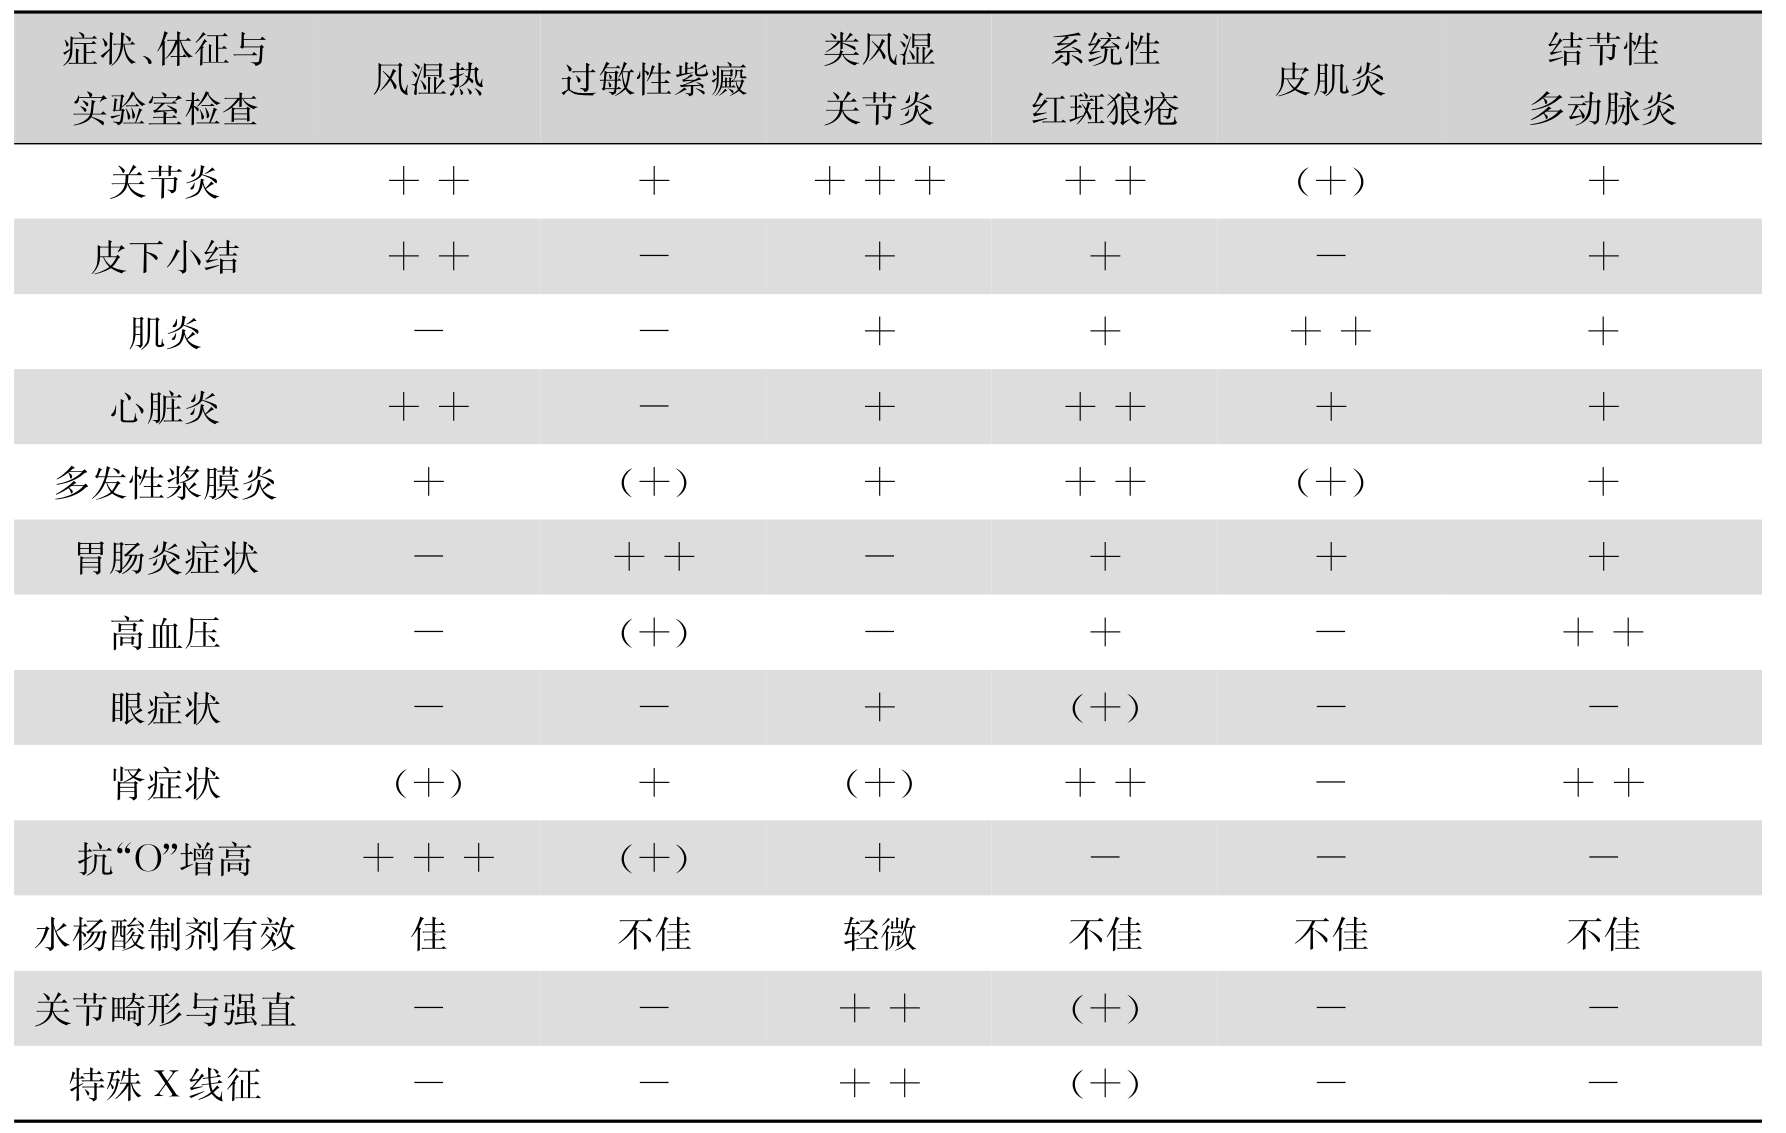
\includegraphics[width=5.94792in,height=3.77083in]{./images/Image00255.jpg}
\end{table}

\protect\hypertarget{text00325.html}{}{}

\section{141 代谢障碍性急性关节炎}

\subsection{一、急性痛风性关节炎}

常见的代谢障碍性急性关节炎是急性痛风性关节炎。

痛风是由单钠尿酸盐沉积所致的晶体相关性关节病,与嘌呤代谢紊乱和(或)尿酸排泄减少所致的高尿酸血症直接相关,特指急性特征性关节炎和慢性痛风石疾病,主要包括急性发作性关节炎、痛风石形成、痛风石性慢性关节炎、尿酸盐肾病和尿酸性尿路结石,重者可出现关节残疾和肾功能不全。主要见于成年男性和更年期以后的女性。有家族病倾向,与食物结构有关,常见于食肉过多及营养丰富者,急性发作常与暴食、酗酒等因素有关。感染、外伤、情绪激动或手术等也可成为急性发作的诱因。

急性发作最初常侵及跖趾关节,其次是足背、踝、手指、膝关节等。肩及髋关节甚少累及。痛风第一次发作多在夜间。开始时常为单个关节发炎,罹患关节呈红、肿、热、痛与运动障碍。急性发作历时数天(一般为3~10天)或数周缓解,关节外形及运动功能也恢复。大多数病例经一段时期后又第二次发作关节肿痛,经反复多次发作后演变为慢性痛风性关节炎,慢性痛风性关节炎的诊断参见第143节。

\subsection{二、假性痛风}

假性痛风是一种由焦磷酸钙二水合物结晶引起的、常累及老年人的关节炎。发病机制未明。本病常累及50岁以上的人,发病率因年龄递增而增加。男女均可罹患。其特征性X线表现是关节软骨的钙化。最常累及膝关节以及其他大关节。曾报告有家族性病例。诊断主要根据病史、X线摄片检查以及罹患关节的滑液检查。在急性发作期,关节滑液中有大量中性粒细胞,焦磷酸钙二水合物结晶常发现于细胞外或中性粒细胞内;在慢性病例中则这些结晶较少见,如有发现,则最常位于中性粒细胞内。本病国内仅见少数报告。

\protect\hypertarget{text00326.html}{}{}

\section{142 原因未明的急性关节炎}

\subsection{一、松毛虫病性关节炎}

本病大多由于集体进入虫害区松山劳动,接触松毛虫或被其污染的松枝、松针、柴草而暴发大、小流行,有时为散发性。起病大多在接触后两天之内,全身症状较轻,而局部症状明显。在多个大、小关节发生肿胀、疼痛与运动障碍,但红肿轻微。疼痛逐渐加剧,可如刀割样。少数病例于局部组织或肌腱形成肿块,逐步增大,经1~2个月消散或溃破自愈。血沉多明显加快。经抗过敏药物及激素治疗后较快康复。少数重症病例演变为慢性,关节变形、肌肉萎缩、功能明显障碍,X线片上显示骨质疏松与破坏、关节间隙不对称性狭窄或消失、骨膜增生。

\subsection{二、血清阴性滑膜炎综合征}

血清阴性滑膜炎综合征也称缓和的血清阴性的对称性滑膜炎伴凹陷性水肿综合征,是一种病因未明、特殊类型的以关节炎为主要表现的风湿性疾病。临床表现为急性对称性、水肿性多关节炎,主要累及老年人,病变多累及手和足关节附近及背侧的肌腱。类风湿因子阴性。X线无骨质侵蚀性改变。此病多呈良性经过,缓解后不遗留功能障碍。

\protect\hypertarget{text00327.html}{}{}

\section{参考文献}

1.辛光宾,等.结核感染过敏性关节炎12例误诊分析.中国实用内科杂志,2001,21(3):179

2.吴宗智.结核感染过敏性关节炎12例治疗体会.现代中西医结合杂志,2004,13(3):372

3.荣风欣,田春辉,荣宁.松毛虫骨关节病1例报告.中国中西医结合影像学杂志,2004,2(4):317

4.王仁崇,等.痛风性关节炎的研究进展.中华风湿病学杂志,2011,15(9):647-650

5.熊焰,等.痛风性关节炎28例临床分析.中华风湿病学杂志,2004,8(3):162-164

6.杨岫岩.风湿性关节炎:一个值得磋商的病名.中华风湿病学杂志,2003,7(1):60-61

7.曾庆馀.血清阴性脊柱关节病诊断治疗新进展.中国实用内科杂志,2000,20(1):50-52

8.李桂叶,安媛,栗占国.缓解性血清阴性对称性滑膜炎伴凹陷性水肿综合征14例临床分析并文献复习.中华风湿病学杂志,2012,16(7):468

9.蒋智铭,张惠箴.焦磷酸钙结晶沉积病(假性痛风)二例.中华病理学杂志,2009,38(12):848-849

10.苏哲坦.反应性关节炎.中华风湿病学杂志,2001,5(1):49-51

\protect\hypertarget{text00328.html}{}{}

